%%%%%%%%%%%%%%%%%%%%%%%%%%%%%%%%%%%%%%%%%%%%%%%%%%%%%%%%%%%%%%%%%%%%%%%%%%%
%%                      Couverture report LaTeX template                 %%
%%%%%%%%%%%%%%%%%%%%%%%%%%%%%%%%%%%%%%%%%%%%%%%%%%%%%%%%%%%%%%%%%%%%%%%%%%%

\documentclass[a4paper,12pt,twoside]{article}
\usepackage{couverture}
\usepackage[T1]{fontenc}
%% \usepackage[french]{babel}
\usepackage[latin1]{inputenc}
\usepackage{url}
\usepackage{amssymb}
\usepackage{amsmath}
\usepackage{subfigure}

\usepackage{tikz}
\usetikzlibrary{arrows,positioning}

\newcommand{\couv}{{\sc Couverture}}
\renewcommand{\le}{\leqslant}
\renewcommand{\ge}{\geqslant}
\newcommand{\N}{\mathbb{N}}
\newcommand{\anysc}{\star}
\newcommand{\andthen}{\texttt{and then}}
\newcommand{\orelse}{\texttt{or else}}
\newcommand{\adanot}{\texttt{not}}

%%%%%%%%%%%%%%%%%%%%%%%%%%%%%%%%%%%%%%%%%%%%%%%%%%%%%%%%%%%%%%%%%%%%%%%%%%%%%%

\newtheorem{theorem}{\textsc{Theorem}}
\newtheorem{definition}{\textsc{Definition}}
\newtheorem{lemma}{Lemma}[subsection]

\def\@begintheorem#1#2{\trivlist
   \item[\hskip \labelsep{#1\ #2}]\itshape}

\begin{document}
\pagestyle{empty}

\vfill

\begin{center}%
{\Large \textbf{\couv{}}}

{\Large \textbf{Technical Report on OBC/MCDC properties}}

\vfill

{\large \textbf{Abstract}}
\end{center}

This document gathers results established or formalized by the \couv{}
project team about relationships between specific coverage criteria.
%
We focus in particular on how \E{Object Branch Coverage} (OBC) relates to the
\E{Modified Condition/Decision Coverage} (MCDC) criterion.

We provide two broad categories of results: formal proofs of important
properties over a model of the two criteria, and a machine-automated
verification of some of these properties for concrete subsets of the model
expressed in Alloy.
%
These results constitute the grounds on which our project coverage analysis
framework operates to infer source coverage results from object coverage
information out of an instrumented execution environment.

\vfill

\newpage
\pagestyle{plain}

%%%%%%%%%%%%%%%%%%%%%%%%%%%%%%%%%%%%%%%%%%%%%%%%%%%%%%%%%%%%%%%%%%%%%%%%%%%%%%

\section{Common definitions}

\subsection{Decisions, conditions}

We are considering decisions that are short circuit boolean expressions,
i.e. expressions consisting in elementary boolean conditions combined
together using only the \andthen{}, \orelse{} and \adanot{} operators.

For each decision we construct the associated ROBDD (Reduced Ordered
Binary Decision Diagram), whose nodes are conditions. (RO)BDDs have an
entry point, and two or more exit edges labeled True and False.

In the remainder of this document, unless otherwise indicated, all
references to BDDs denote reduced ordered BDDs. For a set S, \#S will
refer to this set's cardinal. The following convention will also be
used:

\begin{definition}
  \label{def:general-defs}

  Given a decision D:
  \begin{itemize}
  \item cond(D) will be the set of its conditions;
  \item BDD(D) will be its BDD.
  \end{itemize}
\end{definition}

\subsection{Coverage metrics}

\subsubsection{Definitions}

% define MC/DC, OBC, BDDBC

This document deals with properties of tests exercising object code under
the assumption that the code generation chain accurately preserves the
decision process captured in the ROBDD. We specifically assume when
discussing object branch coverage of the object code, that we can instead
reason, unless indicated explicitly, on (RO)BDD branch coverage
of the corresponding BDD.

\subsection{Minimal test sets}

Coverage assessment is accomplished by exercising some piece of object
code in a variety of test cases, recording data along the way, and
then determining whether the successive executions of the object code
satisfy a given criterion of exhaustiveness. The minimum number of distinct
executions required to achieve a specific criterion is an important
aspect in the evaluation of any coverage assessment methodology. Here
we establish some properties that give a hard limit on test set size
for various coverage metries.

\subsubsection{OBC}

\subsubsection{MC/DC}

\paragraph{Formal definition:}

The formal definition of MC/DC that it used here is the one given
in~\cite{ar0118}, using a graph-coloring algorithm to determine
whether two given evaluations show the independent influence of a
condition. Amongst the various formal definitions that you may find in
the litterature, this one has the advantage to apply also to
short-circuit operators, which is mandatory in the context of \couv{}.

The following will not re-define what has already detailed in~\cite{ar0118};
we will just give an example on how it works and will refer the interested
reader to the original document.

This formal definition of MC/DC uses a simple graph-coloring algorithm
to determine whether two given evaluations show the independent
influence of a condition. it first colors each node of the decision
syntax tree with both evaluations; for example, for a decision
$(A \ \andthen{} \ B) \ \orelse{} \ C'$, the syntax tree can be seen
on figure~\ref{subfig:color-graph-expr}.

\begin{figure}[h]
  \centering

    \subfigure[$(A \ \andthen{} \ B) \ \orelse{} \ C$]{
      \label{subfig:color-graph-expr}

      %        or else
      %       /       \
      %   and then     C
      %  /        \
      % A          B

      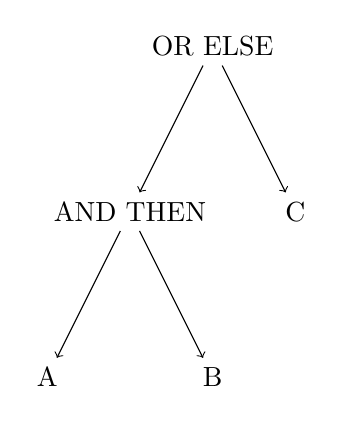
\begin{tikzpicture}[scale=1.4]
	\node (or_else) {OR ELSE}
	child[->] {
	  node (and_then) {AND THEN}
          child[->] {node (and_then_a) {A} edge from parent node[left] {}}
          child[->] {node (and_then_b) {B} edge from parent node[right] {}}
	  edge from parent node[left] {}
	}
	child[->] {node (or_else_c) {C} edge from parent node[right] {}};
      \end{tikzpicture}
    }
\end{figure}

For the evaluation $e1 = (A = True, B = True, C = X)$, we have the
coloring given on figure~\ref{subfig:color-graph-e1}; and for $e2 = (A
= False, B = X, C = False)$, we have the coloring given on
figure~\ref{subfig:color-graph-e2}.

\begin{figure}[h]
  \centering
    \subfigure[e1]{
      \label{subfig:color-graph-e1}

      %        or else T
      %       /       \
      %   and then T   C X
      %  /        \
      % A T        B T

      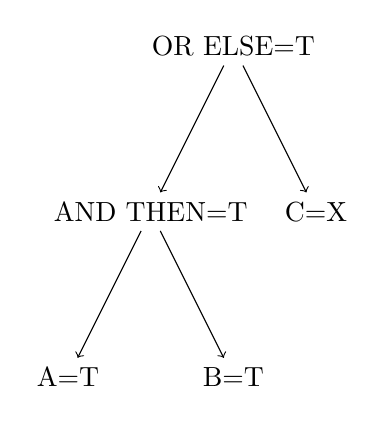
\begin{tikzpicture}[scale=1.4]
	\node (or_else) {OR ELSE=T}
	child[->] {
	  node (and_then) {AND THEN=T}
          child[->] {node (and_then_a) {A=T} edge from parent node[left] {}}
          child[->] {node (and_then_b) {B=T} edge from parent node[right] {}}
	  edge from parent node[left] {}
	}
	child[->] {node (or_else_c) {C=X} edge from parent node[right] {}};
      \end{tikzpicture}
    } \\
    \subfigure[e2]{
      \label{subfig:color-graph-e2}

      %        or else F
      %       /       \
      %   and then F   C F
      %  /        \
      % A F        B X

      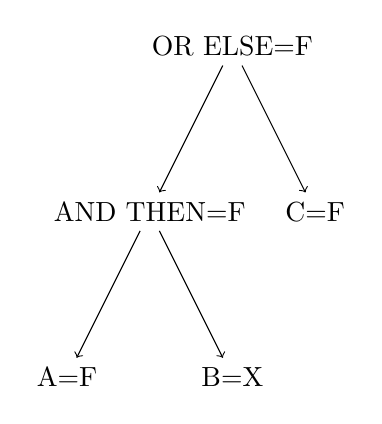
\begin{tikzpicture}[scale=1.4]
	\node (or_else) {OR ELSE=F}
	child[->] {
	  node (and_then) {AND THEN=F}
          child[->] {node (and_then_a) {A=F} edge from parent node[left] {}}
          child[->] {node (and_then_b) {B=X} edge from parent node[right] {}}
	  edge from parent node[left] {}
	}
	child[->] {node (or_else_c) {C=F} edge from parent node[right] {}};
      \end{tikzpicture}
    }
\end{figure}

Both graphs are then combined into an influence tree by xor'ing each
node. An extension of xor to three-value boolean algebra is used:
anything xor Not\_Evaluated gives False. In our case, the result is
showed on figure~\ref{subfig:color-graph-influence-tree}.

\begin{figure}[h]
  \centering
    \subfigure[Influence tree]{
      \label{subfig:color-graph-influence-tree}

      %        or else T
      %       /       \
      %   and then T   C F
      %  /        \
      % A T        B F

      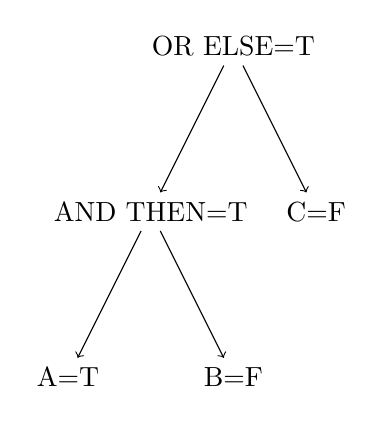
\begin{tikzpicture}[scale=1.4]
	\node (or_else) {OR ELSE=T}
	child[->] {
	  node (and_then) {AND THEN=T}
          child[->] {node (and_then_a) {A=T} edge from parent node[left] {}}
          child[->] {node (and_then_b) {B=F} edge from parent node[right] {}}
	  edge from parent node[left] {}
	}
	child[->] {node (or_else_c) {C=F} edge from parent node[right] {}};
      \end{tikzpicture}
    }
\end{figure}

The influence set of these two evaluations for the given decision is
the set of conditions that have a path of ``True nodes'' to the root.
So here, it is the singleton \{A\}.

The two classical variants of MC/DC are then defined as follow:

\begin{definition}
  \label{def:masking-mcdc}
  Given a decision D, a pair of truth vectors satisfies Masking MC/DC
  for a condition c in cond(D) if and only if its influence set is the
  singleton {c}.

  This decision D satisfies Masking MC/DC if and only if, for each
  condition in cond(D), there exists a pair of tests that satisfies
  Masking MC/DC.
\end{definition}

\begin{definition}
  \label{def:unique-cause}
  Given a decision D, a pair of truth vectors satisfies Unique Cause MC/DC
  for a condition c in cond(D) if and only if its influence set is the
  singleton {c} and if c is the only condition that is colored with True
  in the influence tree.

  This decision D satisfies Unique Cause MC/DC if and only if, for each
  condition in cond(D), there exists a pair of tests that satisfies
  Unique Cause MC/DC.
\end{definition}

In our example, our pair of truth vectors satisfies both Unique Cause and
Masking MC/DC for condition A.

\paragraph{Properties:}

For Unique Cause, the following property holds:

\begin{theorem}
MC/DC on a decision with $n$ independent conditions is achieved with
a test set of exactly $n+1$ tests, and cannot be achieved in fewer tests.
\end{theorem}

The existence of the test set is proved by induction. For one condition,
MC/DC is achieved with two tests, one setting it True and the other False.

Now assume that the property holds for all $n \le{} N$, and consider a decision
with $N+1$ conditions. It is of the form $D = D_l \anysc{} D_r$ where
$\anysc{}$ is either \andthen{} or \orelse{}. There is also possibly a
negation, which is omitted here since it has no impact on MC/DC. For the
remainder of this proof we assume the operator is \andthen{}; the same
reasoning applies similarly for the case of \orelse{}.

$D_l$ and $D_r$ are decisions with respectively $n_l$ and $n_r$ conditions
(both at most $N$), and $n_l + n_r = N+1$. From the induction hypothesis
we have two test vector sets $T_l = \{ v_l (0) .. v_l (n_l) \}$ and
$T_r = \{ v_r (0) .. v_r (n_r) \}$ that satisfy MC/DC for $D_l$ and $D_r$
respectively, and we can arbitrarily choose the indices so that
$D_l$ is True for $v_l(0)$ and $D_r$ is True for $v_r (0)$.

We can now create a combined test set for the complete decision as follows.
$$(\forall j \in [0, n_l])\, v (j) = (v_l (j) \cdot v_r (0))$$
$$(\forall j \in [1, n_r])\, v (n_l + j) = (v_l (0) \cdot v_r (j))$$

We have thus created a set $T = \{ v(0) .. v(n_l + n_r) \}$ of $N+2$ tests.
It is immediate that the elements with indices 0 to $n_l$ give for D
the same outcome as the corresponding elements of $T_l$ for $D_l$,
and they all have identical values for the conditions coming from $D_r$,
so they show independent influence of all conditions coming from $D_l$.
Similarly the vector set $\{v(0), v(n_l+1) .. v(n_l + n_r)\}$ shows
independent influence of those conditions coming from $D_r$, so the new
test set $T$ satisfies MC/DC for $D$ and thus the induction property holds at
$N+1$ as well, since $T$ has $n_l + n_r + 1 = N+2$ elements.

The proof that this is the minimal test set size is given in~\cite{ar0118}.

\subsection{Coverage assessment through analysis of execution traces}


\section{Characterization of cases of BDDBC --- MC/DC equivalence}

This section discusses the distinction between expressions for which
BDDBC of the associated ROBDD implies MC/DC, and expressions for which
no such implication holds.

\subsection{Some cases of non equivalence between OBC and MC/DC}

First let us have a look at how MC/DC and object coverage relate to each
other on some simple cases. Cases of non-equivalence for decisions with up to
5 conditions have been studied in \cite{ar0720}: non-equivalence cases
have been shown to occur in decisions with three or more conditions,
and an illustration is provided with (A \andthen{} B) \orelse{} C,
where A, B and C are three independent conditions.
%
A representation of this decision's BDD is depicted on
figure~\ref{subfig:D1}:

\begin{figure}[h]
\centering

\begin{tabular}{cc}

\subfigure[]{
  \label{subfig:D1}
  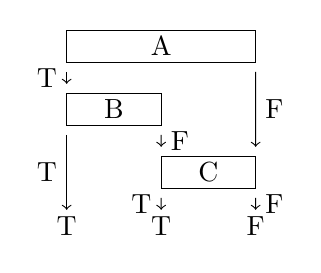
\begin{tikzpicture}[scale=0.8]

    \draw (0,0) rectangle node {A} (3,-0.5);
    \node at (0,-0.5) (if_a_true) {};
    \node at (3,-0.5) (if_a_false) {};

    \draw (0,-1) rectangle node {B} (1.5,-1.5);
    \node at (0,-1)   (b_left) {};
    \node at (1.5,-1)   (b_right) {};
    \node at (0,-1.5) (if_b_true) {};
    \node at (1.5,-1.5) (if_b_false) {};

    \draw (1.5,-2) rectangle node {C} (3,-2.5);
    \node at (1.5,-2)   (c_left) {};
    \node at (3,-2)   (c_right) {};
    \node at (1.5,-2.5) (if_c_true) {};
    \node at (3,-2.5) (if_c_false) {};

    \node at (0, -3) (outcome_true1) {};
    \node at (1.5, -3) (outcome_true2) {};
    \node at (3, -3) (outcome_false) {};

    \node at (0, -3.1) (outcome_true1_label) {T};
    \node at (1.5, -3.1) (outcome_true2_label) {T};
    \node at (3, -3.1) (outcome_false_label) {F};

    \draw [->] (if_a_true)  -- node[left] {T} (b_left);
    \draw [->] (if_a_false) -- node[right] {F} (c_right);

    \draw [->] (if_b_true)  -- node[left] {T} (outcome_true1);
    \draw [->] (if_b_false) -- node[right] {F} (c_left);

    \draw [->] (if_c_true)  -- node[left] {T} (outcome_true2);
    \draw [->] (if_c_false) -- node[right] {F} (outcome_false);

  \end{tikzpicture}
} & \subfigure[]{
  \label{subfig:D2}
  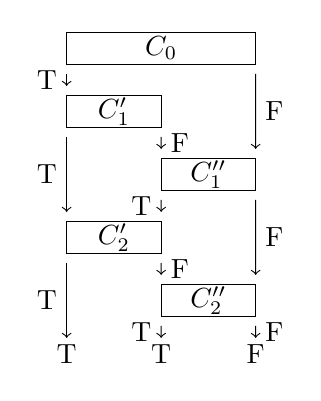
\begin{tikzpicture}[scale=0.8]

    \draw (0,0) rectangle node {$C_{0}$} (3,-0.5);
    \node at (0,-0.5) (if_c0_true) {};
    \node at (3,-0.5) (if_c0_false) {};

    \draw (0,-1) rectangle node {$C'_{1}$} (1.5,-1.5);
    \node at (0,-1)   (c1a_left) {};
    \node at (1.5,-1)   (c1a_right) {};
    \node at (0,-1.5) (if_c1a_true) {};
    \node at (1.5,-1.5) (if_c1a_false) {};

    \draw (1.5,-2) rectangle node {$C''_{1}$} (3,-2.5);
    \node at (1.5,-2)   (c1b_left) {};
    \node at (3,-2)   (c1b_right) {};
    \node at (1.5,-2.5) (if_c1b_true) {};
    \node at (3,-2.5) (if_c1b_false) {};

    \draw (0,-3) rectangle node {$C'_{2}$} (1.5,-3.5);
    \node at (0,-3)   (c2a_left) {};
    \node at (1.5,-3)   (c2a_right) {};
    \node at (0,-3.5) (if_c2a_true) {};
    \node at (1.5,-3.5) (if_c2a_false) {};

    \draw (1.5,-4) rectangle node {$C''_{2}$} (3,-4.5);
    \node at (1.5,-4)   (c2b_left) {};
    \node at (3,-4)   (c2b_right) {};
    \node at (1.5,-4.5) (if_c2b_true) {};
    \node at (3,-4.5) (if_c2b_false) {};

    \node at (0, -5) (outcome_true1) {};
    \node at (1.5, -5) (outcome_true2) {};
    \node at (3, -5) (outcome_false) {};

    \node at (0, -5.1) (outcome_true1_label) {T};
    \node at (1.5, -5.1) (outcome_true2_label) {T};
    \node at (3, -5.1) (outcome_false_label) {F};

    \draw [->] (if_c0_true)  -- node[left] {T} (c1a_left);
    \draw [->] (if_c0_false) -- node[right] {F} (c1b_right);

    \draw [->] (if_c1a_true)  -- node[left] {T} (c2a_left);
    \draw [->] (if_c1a_false) -- node[right] {F} (c1b_left);

    \draw [->] (if_c1b_true)  -- node[left] {T} (c2a_right);
    \draw [->] (if_c1b_false) -- node[right] {F} (c2b_right);

    \draw [->] (if_c2a_true)  -- node[left] {T} (outcome_true1);
    \draw [->] (if_c2a_false) -- node[right] {F} (c2b_left);

    \draw [->] (if_c2b_true)  -- node[left] {T} (outcome_true2);
    \draw [->] (if_c2b_false) -- node[right] {F} (outcome_false);

  \end{tikzpicture}
}\\
\end{tabular}

\caption{Example decision BDDs}
\label{fig:examples}
\end{figure}

From this representation, we can see that a set of three evaluations can
achieve branch coverage of the whole BDD, corresponding to the three vertical
paths in figure~\ref{subfig:D1}.
%
These evaluations are:

\begin{center}
\begin{tabular}{|c|c|c||c|}
\hline
A & B & C & (A \andthen{} B) \orelse{} C \\ \hline
T & T & x & T \\ \hline
T & F & T & T \\ \hline
F & x & F & F \\ \hline
\end{tabular}
\end{center}

where ``x'' means not evaluated and thus can be indifferently True or False.
%
Now, indeed, even though all the BDD edges are covered, MC/DC is not
met. In particular, the independent effect of conditions B on the
decision is not shown in the case of Masking MC/DC, and the
independent effect of both B and C are not shown in the case of Unique
Cause.  Since $n+1$ tests are needed to cover a decision with $n$
condition with respect to MC/DC, 3 evaluations cannot cover a
three-condition decision.

It turns out that this particular case can be generalized in a
quite spectacular counterexample: there exists classes of decisions
with an arbitrary high number of conditions that can be branch covered
by just three evaluations; the previous example was one element of this
class with 3 conditions.

Consider the following set $\{D_{n}\}_{n \in \N}$  of decisions:

\begin{itemize}
\item let $D_{0}$ be a simple condition decision; by convention,
      we will call $C_{0}$ its condition;
\item let us define $D_{n}$, for any $n>0$, as follows:\\
      $D_{n} = (D_{n-1} \ \andthen{} \ C'_{n}) \ \orelse{} \ C''_{n}$\\
      $C'_{n}$ and $C''_{n}$ being independent from each other and from
      any condition in $D_{n-1}$.
\end{itemize}

In other words:
\begin{itemize}
\item $D_{0} = C_{0}$
\item $D_{1} = (C_{0} \ \andthen{} \ C'_{1}) \ \orelse{} \ C''_{1}$
\item $D_{2} = (((C_{0} \ \andthen{} \ C'_{1}) \ \orelse{} \ C''_{1})\\
                 \andthen{} \ C'_{2}) \ \orelse{} \ C''_{2}$
\item $D_{3} = (((((C_{0} \ \andthen{} \ C'_{1}) \ \orelse{} \ C''_{1})\\
                 \andthen{} \ C'_{2}) \ \orelse{} \ C''_{2})\\
                   \andthen{} \ C'_{3}) \ \orelse{} \ C''_{3}$
\item ...
\end{itemize}

Figure~\ref{subfig:D2} shows the BDD for $D_{2}$, where it is visible
that all the edges can be covered by three evaluation paths which only
demonstrate the independent effect of $C_{0}$:

\begin{center}
\begin{tabular}{|c|c|c|c|c||c|}
\hline
$C_{0}$   & $C'_{1}$   & $C''_{1}$   & $C'_{2}$   & $C''_{2}$   & $D_{2}$ \\ \hline
T      & T       & x        & T       & x        & T     \\ \hline
T      & F       & T        & F       & T        & T     \\ \hline
F      & x       & F        & x       & F        & F     \\ \hline
\end{tabular}
\end{center}

We can thus build a decision $D_{n}$ with an arbitrary number of conditions,
that can be BDD branch covered by just three evaluation paths. As MC/DC can
only be achieved with a minimal number of $n+1$ evaluations, this is a
striking case where BDD branch coverage (and consequently OBC) is far from
being equivalent to MC/DC.

We can now adopt a more general perspective and characterize more
precisely the difference between these two criteria.

\subsection{Construction of the ROBDD}

The BDD we associate with a decision is constructed using the following
recursive procedure:

\begin{description}
\item[Build\_BDD.Condition]
  The BDD for a decision consisting in a single condition C has the node
  "test C" as its entry point, the label True is assigned to the branch
  corresponding to "C is True", and the label False is assigned to the
  branch corresponding to "C is False".

\item[Build\_BDD.NOT]
  The BDD for $\adanot{} (D)$ is the BDD for D where the labels of the exit
  edges have been swapped.

\item[Build\_BDD.Short\_Circuit\_Operator]
  This rule defines how the BDD for $(D1) \anysc{} (D2)$ is constructed for
  any short-circuit operator $\anysc{}$.

  If $\anysc{}$ is \andthen{}, let SC be False
  If $\anysc{}$ is \orelse{}, let SC be True

  Let B1 be the BDD for D1, and B2 the BDD for D2.

  Then B, the BDD for D is obtained by combining B1 and B2 as follows:
  \begin{itemize}
    \item the entry point is that of B1
    \item the exit edge labeled SC of B1 is an exit edge labeled SC of B
    \item the other exit edge of B1 connects to the entry point of B2
    \item the exit edges of B2 are exit edges of B with the same labels
  \end{itemize}
\end{description}

The following invariants of ROBDDs follow from the construction process:
\begin{itemize}
  \item There is exactly one BDD node for each condition.
  \item All condition nodes are reachable (i.e. there is a path from
        the entry point to any node in the BDD).
  \item There are no cycles in the BDD.
  \item Both outcomes are reachable (i.e. there is a path from the entry point
        to an exit edge labeled True and to an exit edge labeled False).
\end{itemize}

\subsection{Node ordering}

For a decision D and a condition C in D, let us call index(D,C) the
positive number built by the following recursive procedure:

\begin{description}
\item[Build\_BDD\_Order.Condition]
  The sub-decision is a single condition decision, it is of the form:\\
  $D ::= C$\\
  then index(D,C) = 1\\

\item[Build\_BDD\_Order.NOT]
  The sub-decision is of the form:\\
  $D ::= \adanot{} \ D1$\\
  then for each condition C in D, index(D,C) = index(D1,C)\\

\item[Build\_BDD\_Order.Short\_Circuit\_Operator]
  The sub-decision is of the form:\\
  $D ::= DL \ \anysc{}\ DR$\\
  then, for each condition C in D:\\
  \begin{itemize}
    \item if C is in DL, $index(D,C) = index(DL,C)$
    \item if C is in DR, $index(D,C) = index(DR,C) + \#cond(DL)$
  \end{itemize}
\end{description}

This builds a total order over the conditions of a decision; it is a
general result for reduced order BDD that the reflexive transitive
closure defines a total order over its nodes; this order is the same
as the one we just defined. It can also be demonstrated easily, by
structural induction, that this order is the order of conditions in
the decision's expression.

\subsection{Evaluation of a decision}

Given the transformation of a decision into its ROBDD, evaluating the
decision consists in computing its value using the following BDD traversal
procedure:

\begin{description}
\item[Eval.Condition]
  The value of a decision that consists in a lone condition is the
  value of the condition.

\item[Eval.Not]
  To evaluate $\adanot{} (D)$, evaluate D and take the opposite value

\item[Eval.Short\_Circuit\_Operator]
  To evaluate $(D1) \anysc{} (D2)$, evaluate D1. If $D1 = SC$ then the
  value is SC, else evaluate D2, and the value is that of D2.
\end{description}

The following property holds:

\begin{description}
\item[Evals\_Are\_Paths]
  Evaluating a decision is equivalent to traversing the BDD, evaluating
  each condition as BDD nodes are traversed, and using the label of the
  exit edge as the value of the decision.
\end{description}

This property, and most other properties that we'll discuss here,
is proved by recurrence on the number of binary operators involved in
the expression. We'll assume that it holds for all $n \le{} N$, and then
consider an expression with $N+1$ binary operators, and prove that
the BDD construction step Build\_BDD.Short\_Circuit\_Operator preserves
the property from the two subdecision BDDs to the overall BDD.

Note that the practical implementation of coverage analysis systems based
on control flow traces relies on the assumption that the code generator
used to produce executable code from expressions actually implements this
evaluation strategy.

\subsection{Equivalence case}

We now consider the case of an expression whose BDD has no diamond path,
i.e. for each BDD node there is exactly one path from the entry point to
that node. The following property holds:

\begin{description}
\item[BDDBC\_No\_Diamond\_Indep\_Implies\_MCDC]
  For a BDD with no diamond, if conditions are independent, then
  BDD branch coverage implies masking MC/DC coverage.
\end{description}

Let's consider a condition C. Since we have BDD branch coverage,
all possible paths starting at C have been taken (by recurrence on path
length, taking advantage of no cycles and no diamonds).

From the independent outcome reachability property, we have two paths
starting at C, beginning each with one edge from C, and ending on the
two outcomes of the decision. Let's call them PCT and PCF.

These paths are disjoint: any condition appearing in one is masked
in the other (because of no-diamond).

These two paths are parts of paths PT and PF from the BDD entry point to
either outcome, and they cannot differ on the part of the path from the
entry point to C.

So, PT and PF differ in C, in no other condition before C, and in no
other non-masked condition after C, so they prove independent influence
of C over the decision.

This holds for each condition in the decision, so MC/DC is proved.

\subsection{Non-equivalence case}

The general idea of this proof is to show that, for any BDD with a
diamond, we can build a set of evaluations that covers the BDD
branches in such a way that there is at least one condition for which
MC/DC is not met.

If we want to have a proof that will work for any definition of MC/DC,
we cannot rely on a failure of the independence criteria; \textit{to
independently affect} means something different in unique cause MC/DC
or in masking MC/DC. So we should rather rely, if it is possible, on
the set of properties that these criteria have in common; a sort of
\textit{greatest common divisor} of the two criteria. Let us define
this weak MC/DC criteria as follow:

\begin{itemize}
\item every possible outcome of the decision have been tried;
\item each condition in the decision has taken on every possible outcome;
\item each condition in the decision is shown to affect the outcome of the
      decision.
\end{itemize}

The only difference with MC/DC here is that weak MC/DC does not care
if the condition \textit{independently} affects the outcome of the decision;
whatever \textit{independently} means. Weak MC/DC is weaker than any other
MC/DC criteria. So, if a set of evaluations does not satisfy weak MC/DC,
it won't satisfy unique cause MC/DC or masking MC/DC.

The formal definition would be:

\begin{definition}
  \label{def:weak-mcdc}
  Given a decision D, a pair of truth vectors satisfies weak MC/DC for
  a condition c if and only if, in their influence tree, the node c
  and the root node are both colored in True.

  This decision D satisfies weak MC/DC if and only if, for each
  condition in cond(D), there exists a pair of tests that satisfies
  weak MC/DC.
\end{definition}

It turns out that we can build a set of evaluations such that BBDBC is
reached, but not MC/DC, when the BDD has a diamond.  Let's take the
canonical example: $(A \ \andthen{} \ B) \orelse{} \ C$, and these
evaluations:

\begin{center}
\begin{tabular}{|c|c|c||c|}
\hline
A & B & C & (A \andthen{} B) \orelse{} C \\ \hline
T & T & x & T \\ \hline
T & F & T & T \\ \hline
F & x & F & F \\ \hline
\end{tabular}
\end{center}

This set covers this decision for BDDBC. However, this does not meet
weak MC/DC; whenever B is evaluated, the decision outcome is True. So
this cannot show that B affects the outcome of the decision.

Let us give a general idea of how we would prove that in the general
case. First, remember that we are dealing with reduced ordered BDDs;
so each node can be ordered. This property allows us to have a
proper concept of ``last diamond node'' and its ``last parent''. In our
example, the last diamond node would be C, its last parent B.

Now, we would show that the last parent of the last diamond node has
an interesting property: one of its exit edge is always connected
directly to an outcome (for B, it is outcome True). Its other exit
edge being connected to the last diamond node (obviously), it is
possible to cover this edge in such a way that the outcome of the
corresponding evaluation is the same as the ``direct outcome'';
e.g. when evaluating B to False, we would evaluate C to True and exit
on True. We know that this is possible using the property that, from
each node of the BDD (and, in this case, the diamond C), there exists
at least one evaluation that reaches outcome True and at least one that
reach outcome False.

This means that we can cover all exit and incoming edges of the last
parent of the last diamond in such a way that the evaluations \textit{always}
exit on the same outcome; and, from the property of its exit edges, we
can see that this set of evaluations can be completed to reach BDDBC
\textit{without evaluating this node anymore}. This builds a BDD coverage
that does not satisfy weak MC/DC for this node.

The following sections will detail this proof.

\subsubsection{Last diamond}

We have previously built a function index(D,C) that defines a full
order over the nodes of a (RO)BDD. Based on this function, we can
define the following entities:
\begin{itemize}
\item in a BDD, let the last node be the node with the greatest index;
\item let a diamond node be a node with more than one parent;
\item let the last diamond node of a decision be the diamond with the
      greatest index;
\item let the last parent of a node be the parent with the greatest index.
\end{itemize}

Some examples from our canonical case
$D ::= (A \ \andthen{} \ B) \orelse{} \ C$:
\begin{itemize}
\item index(D,A) = 1, index(D,B) = 2, index(D,C) = 3;
\item the last diamond node is C; it is also the last node;
\item the last parent of C is B.
\end{itemize}

We have the following properties:

\begin{lemma}
  \label{lemma:last-node}
  The two exit edges of the last node are connected to both outcomes.
\end{lemma}

\begin{lemma}
  \label{lemma:last-parent-of-the-last-diamond}
   If a BDD contains diamonds, then the last parent of the last diamond
   has an exit edge that is directly connected to an outcome.
\end{lemma}

This can be seen in our example:
\begin{itemize}
\item the last node being C, its exit edges are connected directly to True and
      False;
\item the last parent of the last diamond being B; when it is True, the outcome
      True is reached.
\end{itemize}

The two properties can be proven by structural induction on the BDD.
The first is the easiest one and we will let it as an exercice for the
reader. Here is a proof of the second one:

\begin{itemize}
\item if $D ::= C$ (simple condition decision):\\
  the BDD does not contain any diamond, so the property is trivially true
  in this case.

\item if $D ::=\ \adanot{} \ D1$:\\
  if D1 does not contains diamond, D does not either, the propery is trivial
  as well. If it does contain diamond, well, only outcome labels are different
  between BDD(D) and BDD(D1), so the property holds for D if it holds for D1.

\item if $D ::= DL \ \anysc{} \ DR$, supposing that the property holds
  for DL and DR; four cases then:

  \begin{itemize}
  \item If no diamonds were in BDD(DL) and BDD(DR), and none were introduced
    by building BDD(D) from them: then BDD(D) contains no diamonds, the
    property is trivial.

  \item If DR contains a diamond: then the last diamond node of D is
    the last diamond node in DR. By construction, BDD(DR) is a
    sub-tree of BDD(D), the exit edges of the last diamond node are
    the same in BDD(DR) and in BDD(D). So if the property holds for
    DR, it holds for D.

  \item If DR contains no diamonds, and if building BDD(D) from
    BDD(DR) and BDD(DL) introduces a new diamond: this new diamond
    node has to be root(DR), as only this node has gained new incoming
    edges: in Build\_BDD, the exit edges of BDD(DR) labeled ``not SC''
    are connected to BDD(DL)'s root. Therefore, its parent nodes are
    all in cond(DL). And the last node of BDD(DL) is one of these
    parent nodes; by property~\ref{lemma:last-node}, it has an exit
    edge to ``not SC'' in BDD(DL). Its other exit edge will remain
    unchanged in BDD(D) and will be connected to an outcome
    (``SC''). This last node of BDD(DL) is also the last parent of
    this diamond node, as no other nodes in cond(DL) have an greater
    index. And (finally), this introduced diamond node is D's last
    diamond node, as DR contains no diamonds (initial hypothesis). So
    we have identified the last parent of the last diamond and showed
    that one of exit edge is connected to an outcome in BDD(D); that's
    the property that we were trying to prove.

  \item If DR contains no diamonds, and if no diamonds were introduced
    when building BDD(D), but if DL contains a diamond: the last
    diamond node in D is the same node as the last diamond node in DL.
    The last parent of the last diamond in DL has an exit edge that
    connects to SC; otherwise, it would be connected to BDD(DR)'s root
    when building BDD(D), and as the last node would also be connected
    to this root node (it also has an exit edge to SC in DR, as a
    consequence of property~\ref{lemma:last-node}), BDD(DR)'s root
    would have at least two fathers in D, which contradicts the
    hypothesis that no diamonds were introduced. So this exit edges of
    the last parent of the last diamond in DL (and D) will still be
    connected to an outcome after building D. So the property is true
    in this case as well.
  \end{itemize}
\end{itemize}

The property~\ref{lemma:last-parent-of-the-last-diamond} has now been
established in all possible cases. This proof will actually be quite
useful as its structure will be used to build a coverage that satisfies
BBDBC but not Weak MC/DC.

\subsubsection{Path though BDDs - Conventions}

Some conventions first to help us manipulate paths through BDD:

\begin{itemize}
\item For two paths pl, pr into two different BDDs,
  concat(pl, pr) is the concatenation of these two paths obtained by replacing
  the outcome of pl by the first node in pr.

\item For two set of paths PL, PR through two different BDDs, merge(PL, PR)
  is the set built by doing an arbitrary mapping of each element
  of PL to each element of PR, and concatenating each pair; as these
  two sets may not have the same number of elements, all the remaining
  elements of the greatest set will be mapped to one arbitrary element
  of the smallest set.

\item For any set of paths PS through a BDD (each going from the root node to
  an outcome), let us call path\_to(True, PS) the subset of paths reaching
  outcome True, and path\_to(False, PS) the subset reaching False. We have
  the obvious property:

  $PS = path\_to(True, PS) + path\_to(False, PS)$
\end{itemize}

\subsubsection{Building a BDD branch coverage that does not verify Weak MC/DC}

For a given decision D, our coverage will be ensured by the union of
three sets of paths Short\_Circuit\_LPLD(D), Long\_Circuit\_LPLD(D) and
LPLD\_Not\_Evaluated(D), which verifies the following set-specific
invariants:

\begin{description}
\item[Short\_Circuit\_LPLD\_Invariant]
  If BDD(D) is diamondless, Short\_Circuit\_LPLD(D) is empty;
  otherwise, it contains a non-empty set of paths, each reaching the
  last parent of the last diamond node and then exiting on its direct
  outcome.

\item[Long\_Circuit\_LPLD\_Invariant]
  If BDD(D) is diamondless, Long\_Circuit\_LPLD(D) is empty;
  otherwise, it contains a non-empty set of paths, each reaching the last
  parent of the last diamond node, then going to the last diamond node, and
  then reaching the same outcome as Short\_Circuit\_LPLD(D).

\item[LPLD\_Not\_Evaluated\_Invariant]
  No path in LPLD\_Not\_Evaluated(D) evaluates the last parent of the last
  diamond node.
\end{description}

...plus one other ``global'' invariants:

\begin{description}
\item[BDDBC\_Coverage\_Invariant]
 The union of these three sets covers each edges of the considered
 BDD.
\end{description}

As a consequence of this last invariant, we will now call
BDDBC\_Coverage the union of these three sets:

  $BDDBC\_Coverage(D) = Short\_Circuit\_LPLD(D)\\
                         + Long\_Circuit\_LPLD(D) + LPLD\_Not\_Evaluated(D)$

Note also that an other property falls naturally from
LPLD\_Not\_Evaluated\_Invariant and BDDBC\_Coverage\_Invariant:

\begin{description}
\item[Incoming\_Edges]
  The union of Long\_Circuit\_LPLD and Short\_Circuit\_LPLD covers all incoming
  edges of the last parent of the last diamond node.
\end{description}

Anyway, here is the definition, case by case, of a recursive build
procedure that builds such sets from a decision D. It assumes that all
its sub-decisions have such sets verifying these invariants (not
considering D as a sub-decision of D, obviously; ``strict'' sub-decisions):

\begin{description}
\item[Build\_BDD\_Cov.Condition]
  The sub-decision is a single condition decision, it is of the form:\\
  $D ::= C$

  In this case:
  \begin{itemize}
  \item $Short\_Circuit\_LPLD(D) = Long\_Circuit\_LPLD(D) = \{\}$
  \item $LPLD\_Not\_Evaluated(D) = \{C -> True, C -> False\}$
  \end{itemize}


\item[Build\_BDD\_Cov.NOT]
  The sub-decision is of the form:\\
  $D ::=\ \adanot{} \ D1$

  Then Short\_Circuit\_LPLD(D) is built by switching the outcome of each
  path contained in Short\_Circuit\_LPLD(D1). Same operations for
  Long\_Circuit\_LPLD(D) and No\_LPLD(D).


\item[Build\_BDD\_Cov.Short\_Circuit\_Operator]
  The sub-decision is of the form:\\
  $D ::= DL \anysc{} DR$

  Four sub-cases:

  \begin{itemize}
  \item No diamonds:\\
    No diamonds in BDD(DL) and BDD(DR), and none were introduced
    by building BDD(D) from them. Then:\\
    \begin{itemize}
    \item $Short\_Circuit\_LPLD(D) = \{\}$
    \item $Long\_Circuit\_LPLD (D) = \{\}$
    \item $LPLD\_Not\_Evaluated(D) = path\_to(SC, BDDBC\_Coverage(DL))\\
      + merge(path\_to(not SC, BDDBC\_Coverage (DL)),\\
      BDDBC\_Coverage(DR))$
    \end{itemize}

  \item Diamond in DR:\\
    i.e. Short\_Circuit\_LPLD(DR) and Long\_Circuit\_LPLD(DR) contain at least
    one element each.
    Let p\_dl be an arbitrary path to ``not SC'' in BDD(DL), taken from
    BDDBC\_Coverage(DL). In BDD(D), it corresponds to a path to root(DR).
    Then:
    \begin{itemize}
    \item $Short\_Circuit\_LPLD(D) = merge({p\_dl},\\
                                     Short\_Circuit\_LPLD(DR))$
    \item $Long\_Circuit\_LPLD(D)  = merge({p\_dl},\\
                                        Long\_Circuit\_LPLD(DR))$
    \item $LPLD\_Not\_Evaluated(D) = path\_to(SC, BDDBC\_Coverage(DL))\\
                            + merge(path\_to(not SC, BDDBC\_Coverage(DL)),\\
                            LPLD\_Not\_Evaluated(DR))$
    \end{itemize}
  
  \item Last diamond introduced:\\
    i.e. no diamonds in BDD(DR) and a diamond has been created when building
    BDD(D). In this case:
    \begin{itemize}
    \item $Short\_Circuit\_LPLD(DR) = Long\_Circuit\_LPLD(DR) = \{\}$
    \item the last diamond node in D is root(DR).
    \end{itemize}

    Let SC\_DL be the subset of paths in path\_to(SC,
    BDDBC\_Coverage(DL)) that evaluates the last node in BDD(DL).
    Similarly, let LC\_DL be the subset of paths in path\_to(not SC,
    BDDBC\_Coverage(DL) that evaluates the last node in BDD(DL); in
    BDD(D), this one corresponds to a path to root(DR).  Let $REST\_DL
    = BDDBC\_Coverage(DL) - (SC\_DL + LC\_DL)$ be the subset of paths
    in BDDBC\_Coverage(DL) that do not evaluates this last node.  Let
    sc\_dr be an arbitrary path in DR exiting on SC.

    Then the coverage for BDD(D) is built as follows:
    \begin{itemize}
    \item $Short\_Circuit\_LPLD(D) = SC\_DL$
    \item $Long\_Circuit\_LPLD(D)  = merge(LC\_DL, {sc\_dr})$
    \item $LPLD\_Not\_Evaluated(D) = path\_to(SC, REST\_DL)\\
                            + merge(path\_to(not SC), REST\_DL),\\
                            BDDBC\_Coverage(DR))$
    \end{itemize}
    (Note that we are allowed to merge path\_to(not SC, REST\_DL) because
    it is non-empty; there is at least one other node that has an exit
    edge directly connected to ``not SC'' in BDD(DL), otherwise no
    diamond would have been created; so it must have at least one path
    that does not evaluate the last node in BDD(DL); that property
    gives us the right to use the merge operation. Same thing for LC\_DL
    and SC\_DL that are both non-empty thanks to Last\_Node property).

  \item Diamond in DL only:\\
    i.e. no diamonds in BDD(DR), no new diamonds introduced when
    building BDD(D), but at least one diamond in BDD(DL).  The last
    parent of the last diamond in DL has its ``direct'' exit edge
    that connects to SC; otherwise, it would have been connected to
    BDD(DR)'s root when building BDD(D), and as the last node would
    also be connected to this root node (it also has an exit edge to
    SC in DR, as a consequence of property Last\_Node), BDD(DR)'s
    root would have at least two fathers in D, which contradicts the
    hypothesis that no diamonds were introduced.  Let sc\_dr be an
    arbitrary path in DR exiting on SC.  Then the coverage for BDD(D)
    is built as follows:
    \begin{itemize}
    \item $Short\_Circuit\_LPLD(D) = Short\_Circuit\_LPLD(DL)$
    \item $Long\_Circuit\_LPLD(D)  = merge(Long\_Circuit\_LPLD, {sc\_dr})$
    \item $LPLD\_Not\_Evaluated(D) = path\_to(SC, LPLD\_Not\_Evaluated(DL))\\
                           + merge(path\_to(not SC, LPLD\_Not\_Evaluated(DL),\\
                           BDDBC\_Coverage(DR))$
    \end{itemize}
  \end{itemize}
\end{description}

It is quite easy to check that Short\_Circuit\_LPLD\_Invariant,
Long\_Circuit\_LPLD\_Invariant, LPLD\_Not\_Evaluated\_Invariant and
BDDBC\_Coverage\_Invariant are enforced by this build procedure; each
one falls so obviously from the construction (in every case) that
it will be quite painful to elaborate.

So we can build a BDD coverage in such a way that, if there is a
diamond in the BDD, then the decision will have the same outcome for
any evaluation where the last parent of the last diamond is
evaluated. This means that this BDD coverage does not imply weak
MC/DC; that which was to be demonstrated.

\subsection{Conclusion}

We have therefore proved the following property:

\begin{theorem}
  \label{thm:no-diamond}
  Given a decision D, branch coverage of the BDD implies MC/DC if,
  and only if, there is no diamond in the BDD (i.e.  no node of the
  BDD is reachable through more that one path from the root).
\end{theorem}

Intuitively, BDDBC is a local property of BDD traversals (i.e. of evaluations
of the decision): it is evaluated individually for each BDD node, without
respect to how the BDD node was reached. In contrast, MC/DC is a non-local
property, since it involves the complete path through the BDD. To establish
independent influence of condition C, it is necessary to study what happens
for two values of C leading to different outcomes, \emph{with all other
conditions fixed}, i.e. considering a single way of \emph{arriving to C}.

\section{A second characterization of the equivalence case}

In this section we provide an alternative (equivalent) property
that characterizes cases where BDD branch coverage implies MC/DC:

\begin{theorem}
  \label{thm:lhs-same-operator}
  Given a decision D, BDD branch coverage implies MC/DC if, and only if, when
  considering the negation normal form D' of D, for every sub-decision E of D',
  all binary operators in the left-hand-side operand of E, if any, are of the
  same kind as E's operator.
\end{theorem}

The negative normal form is obtained by rewriting the expression using
De Morgan's laws so that negations apply only to atomic conditions (and not
to more complex subexpressions).

We prove this theorem by showing that this alternative characterization is
equivalent to having no diamond in the associated BDD.
Theorem~\ref{thm:lhs-same-operator} follows by application of
Theorem~\ref{thm:no-diamond}.

Let's consider a decision D and its BDD. For the order of atoms in the
BDD, we take the order in which they appear in a depth-first traversal
of the decision (represented as a tree).

% ??? Add results about ordering...

\begin{figure}
\centering

\subfigure[$DL \ \orelse{} \ DR$]{
\label{subfig:DL-or-DR}
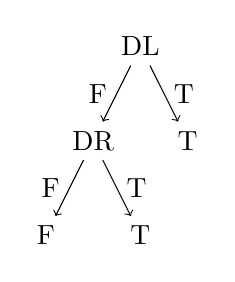
\begin{tikzpicture}[scale=0.8]
  \node (DL) {DL}
    child[->] {
      node (DR) {DR}
        child[->] {node (DRF) {F} edge from parent node[left] {F}}
        child[->] {node (DRT) {T} edge from parent node[right] {T}}
      edge from parent node[left] {F}
    }
    child[->] {node (DLT) {T} edge from parent node[right] {T}};
\end{tikzpicture}

%           DL
%        F / \ T
%         /   \
%        DR    T
%     F / \ T
%      /   \
%     F     T

}
\subfigure[$DL \ \andthen{} \ DR$]{
\label{subfig:DL-and-DR}
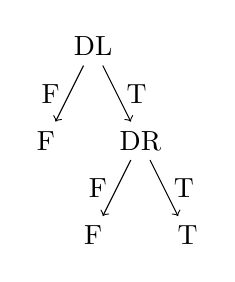
\begin{tikzpicture}[scale=0.8]
  \node (DL) {DL}
    child[->] {node (DLF) {F} edge from parent node[left] {F}}
    child[->] {
      node (DR) {DR}
        child[->] {node (DRF) {F} edge from parent node[left] {F}}
        child[->] {node (DRT) {T} edge from parent node[right] {T}}
      edge from parent node[right] {T}
    };
\end{tikzpicture}

%           DL
%        F / \ T
%         /   \
%        F     DR
%           F / \ T
%            /   \
%           F     T

}
\caption{case 2 and 3}
\end{figure}

There is a diamond in a BDD if and only if there is at least one node
such that the number of paths to reach it from root is strictly
greater than 1; we will use this caracterization to prove our
property.

\emph{Proof of the simplified case:}

Consider first the case where decision D does not contain any negation.
Each non-terminal node in the BDD corresponds to a sub-decision D' in D
(i.e. the root of each sub-decision is a non-terminal node in D's BDD).

\emph{Proof of reverse implication (simplified case):}

Let's call NF(D) the number of paths from the root of decision D to False (F)
and NT(D) the number of paths from the root of decision D to True (T).

\emph{case 1:} D = A (atom)\\
$NF(D) = NT(D) = 1$

\emph{case 2:} D = $DL \ \orelse{} \ DR$\\
The BDD for D can be constructed from the BDDs for DL and DR. It is shown 
in Figure~\ref{subfig:DL-or-DR}.


$NF(D) = NF(DL) * NF(DR)$\\
$NT(D) = NT(DL) + NF(DL) * NT(DR)$

\emph{case 3:} D = $DL \ \andthen{} \ DR$\\
The BDD for D can be constructed from the BDDs for DL and DR. It is shown 
in Figure~\ref{subfig:A-and-B}.

$NF(D) = NF(DL) + NT(DL) * NF(DR)$\\
$NT(D) = NT(DL) * NT(DR)$

\begin{lemma}
\label{lemma:NF-NT-bound}
For every E, $NF(D) \ge 1$ and $NT(D) \ge 1$.
If D is of the form \orelse{} then $NT(D) \ge 2$.
If D is of the form \andthen{} then $NF(D) \ge 2$.
\end{lemma}

\begin{lemma}
\label{lemma:NF-NT-monotonic}
NF and NT are monotonic functions, i.e. if D' is a sub-decision of D,
then we have
        $NF(D') \le NF(D)$
and        
        $NT(D') \le NT(D)$.
\end{lemma}

Proofs of Lemmas~\ref{lemma:NF-NT-bound} and~\ref{lemma:NF-NT-monotonic} are on
structural induction on the form of decisions, based on the three cases
distinguished above.

Then, suppose a decision D of the form \andthen{} contains a
sub-decision D' of the form \orelse{} on the left-hand side, of the form
\orelse{}. If DL, DR are the two sub-decisions such that
$D = DL \andthen{} DR$, then D' is also a sub-decision of DL.

By Lemma~\ref{lemma:NF-NT-bound}, we know that $NT(D') \ge 2$. By
Lemma~\ref{lemma:NF-NT-monotonic}, we know that $NT(DL) \ge NT(D')$.

Then, in D's BDD, the paths reaching the DR's root node are exactly
those paths in DL's BDD reaching True, by construction; the number of
these paths is NT(DL).

Thus, DR's root node in the D's BDD is reachable by more than one
path. As a consequence, there is a diamond in this BDD.

Similarly, if a decision D of the form \orelse{} contains a
sub-decision D' of the form \andthen{} on the left-hand side, we can
exhibit a non-terminal node in the BDD for D that is reachable by more
than one path.

By contraposition, if there are no diamonds in the BDD associated to a
decision D, then D has no \orelse{} sub-decision on the left of its
\andthen{} sub-decisions, and no \andthen{} sub-decision to the left of
its \orelse{} sub-decision.

\emph{Proof of implication (simplified case):}

Now suppose that for every sub-decision in decision D, the left
operand of an \andthen{} sub-decision contains only \andthen{}
sub-decisions and the left operand of an \orelse{} sub-decision
contains only \orelse{} sub-decisions.

\begin{lemma}
\label{lemma:NF-NT-only-one-oper}
If E contains only \orelse{} sub-decisions then $NF(E) = 1$.
If E contains only \andthen{} sub-decisions then $NT(E) = 1$.
\end{lemma}

Proof of Lemma~\ref{lemma:NF-NT-only-one-oper} is on structural induction on
the form of decisions, based on the 3 cases distinguished above.

By structural induction on the depth of the BDD, we can show that there cannot
be any diamond in the BDD associated to D, which proves that the desired
implication holds.

\emph{Proof of the general case:}

In the general case, decision D may contain \adanot sub-decisions. Then,
consider D' the negation normal form of D. Since D and D' are represented
by the same BDD, Theorem~\ref{thm:lhs-same-operator} follows.

\section{General stateless MC/DC assessment}

This section discusses a code transformation after which stateless BDDBC
traces carry sufficient information to assess MC/DC coverage.

\section{Automated verifications}

\newpage
\bibliographystyle{alpha}
\bibliography{couverture}

\end{document}
